\documentclass[notes]{beamer}       % print frame + notes
%documentclass[notes=only]{beamer}   % only notes
%\documentclass{beamer}              % only frames

\usetheme{Copenhagen}
\usecolortheme{beaver}

\setbeamertemplate{navigation symbols}{}

\setbeamertemplate{frametitle}[default][center]

\usepackage{biblatex}
\bibliography{main}

\usepackage{hyperref}
\usepackage{minted}
\usepackage{amsmath}
\usepackage{multicol}
\usepackage{bibentry}
\usepackage{booktabs}
\usepackage{standalone}
\usepackage{annotate-equations}
\usepackage[normalem]{ulem}

\usepackage{graphicx}
\usepackage{tikz}

\usetikzlibrary{calc, patterns}

\tikzstyle{level 1}=[level distance=3.5cm, sibling distance=3.5cm]
\tikzstyle{level 2}=[level distance=3.5cm, sibling distance=2cm]
\tikzstyle{level 3}=[level distance=3.5cm, sibling distance=1cm]
\tikzstyle{player} = [text width=5em, draw, text centered, rectangle, fill=blue!20, inner sep=1pt]
\tikzstyle{nature} = [minimum width=3pt,circle,  draw, fill=red!20, inner sep=1pt]
\tikzstyle{end} = [circle, minimum width=3pt, fill, inner sep=0pt, right]
\tikzstyle{vertex} = [draw, shape=circle, minimum width=.3cm, inner sep=.5pt]

\title{Matching Games, Routing Games and Cooperative Game Theory}
\author{Vince Knight}
\date{}


\begin{document}

\frame{
    \titlepage
}

\section{knightva@cardiff.ac.uk}

\begin{frame}
    \centering

    \includegraphics[height=2cm]{static/CUident_CMYK.png}
    \hfill
    \includegraphics[height=2cm]{static/Logo_UNAM_Namibia.png}\\
    \tiny{2024-03-04 until 2024-03-29}

\end{frame}

\begin{frame}
    \centering

    \includegraphics[height=5cm]{static/swakopmund.jpg}
    \hfill
    \includegraphics[height=5cm]{static/dune_at_sunset.jpg}
\end{frame}


\begin{frame}
    \centering
    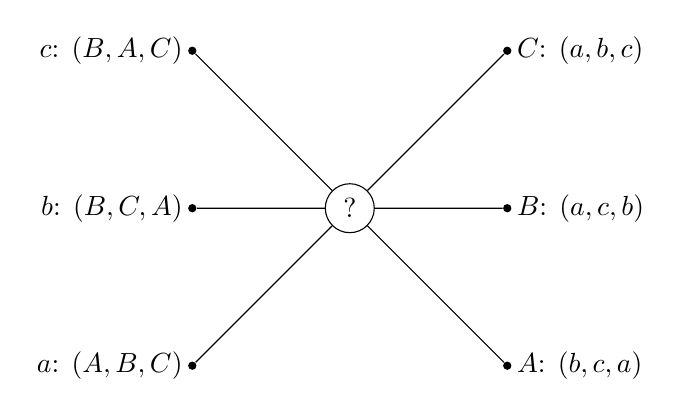
\begin{tikzpicture}[scale=2]
        \node (a) [end] at (0,0) {};
        \node (b) [end] at (0,1) {};
        \node (c) [end] at (0,2) {};
        \node (A) [end] at (2,0) {};
        \node (B) [end] at (2,1) {};
        \node (C) [end] at (2,2) {};
        \node [left] at (a) {$a$: $(A,B,C)$};
        \node [left] at (b) {$b$: $(B,C,A)$};
        \node [left] at (c) {$c$: $(B,A,C)$};
        \node [right] at (A) {$A$: $(b,c,a)$};
        \node [right] at (B) {$B$: $(a,c,b)$};
        \node [right] at (C) {$C$: $(a,b,c)$};
        \node (?) [circle,draw] at ($(B)!0.5!(b)$) {?};
        \draw (A) -- (?);
        \draw (B) -- (?);
        \draw (C) -- (?);
        \draw (a) -- (?);
        \draw (b) -- (?);
        \draw (c) -- (?);
    \end{tikzpicture}
\end{frame}

\note{
    Let us start with a slightly different type of game.

    The set of small letters on the left wants to be matched with the sets of
    small letter on the right.

    Each of their preference is indicated in the brackets. For example \(a\)
    would prefer to be matched with \(A\) over \(B\) over \(C\).

    Can you identify a potential matching?
}

\section{Matching Games}

\frame{
    \begin{definition}
        A matching game of size \(N\) is defined by two disjoint sets \(S\) and
        \(R\) or suitors and reviewers of size \(N\). Associated to each element of
        \(S\) and \(R\) is a preference list:

        \[f:S\to R^N\text{ and }g:R\to S^N\]

    \end{definition}
}

\note{So this is a formal definition of the situation we had above.

We had \(N=3\).

\[S=\{a, b, c\}\]

and 

\[R=\{A, B, C\}\]
}

\frame{
    \begin{definition}
        A matching \(M\) is any bijection between \(S\) and \(R\). If \(s\in S\)
        and \(r\in R\) are matched by \(M\) we denote:

        \[M(s)=r\]
    \end{definition}
}

\note{
    Here is our formal definition of what we are looking for: a matching.
}

\frame{
    
\centering
\begin{tikzpicture}[scale=2]
    \node (a) [end] at (0,0) {};
    \node (b) [end] at (0,1) {};
    \node (c) [end] at (0,2) {};
    \node (A) [end] at (2,0) {};
    \node (B) [end] at (2,1) {};
    \node (C) [end] at (2,2) {};
    \node [left] at (a) {$a$: $(A,B,C)$};
    \node [left] at (b) {$b$: $(B,C,A)$};
    \node [left] at (c) {$c$: $(B,A,C)$};
    \node [right] at (A) {$A$: $(b,c,a)$};
    \node [right] at (B) {$B$: $(a,c,b)$};
    \node [right] at (C) {$C$: $(a,b,c)$};
    \draw (a) -- (A);
    \draw (b) -- (B);
    \draw (c) -- (C);
\end{tikzpicture}
}

\note{
    Here is a matching.

    If you look closely you might notice that there is some instability here.

    \(c\) would prefer to be matched with \(B\) over their current matching
    \textbf{and} \(B\) would prefer to be matched with \(c\) over their current
    matching.
}

\frame{
    \begin{definition}
        A pair \((s,r)\) is said to \textbf{block} a matching \(M\) if \(M(s)\ne r\)
        but \(s\) prefers \(r\) to \(M(r)\) and \(r\) prefers \(s\) to
        \(M^{-1}(r)\).
    \end{definition}
}

\note{
    In the case of the proposed matching \((c,B)\) is a blocking pair.
}

\frame{
    \centering
    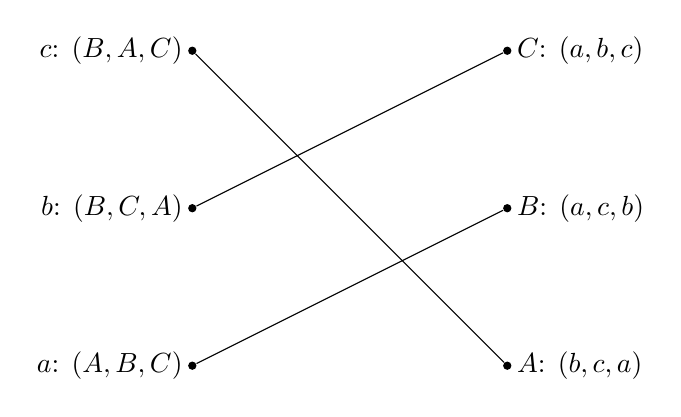
\begin{tikzpicture}[scale=2]
        \node (a) [end] at (0,0) {};
        \node (b) [end] at (0,1) {};
        \node (c) [end] at (0,2) {};
        \node (A) [end] at (2,0) {};
        \node (B) [end] at (2,1) {};
        \node (C) [end] at (2,2) {};
        \node [left] at (a) {\(a\): \((A,B,C)\)};
        \node [left] at (b) {\(b\): \((B,C,A)\)};
        \node [left] at (c) {\(c\): \((B,A,C)\)};
        \node [right] at (A) {\(A\): \((b,c,a)\)};
        \node [right] at (B) {\(B\): \((a,c,b)\)};
        \node [right] at (C) {\(C\): \((a,b,c)\)};
        \draw (c) -- (A);
        \draw (a) -- (B);
        \draw (b) -- (C);
    \end{tikzpicture}
    }

    \note{
        This is a stable matching. 

        Can we always find one?
    }

\frame{
    \centering
    \includegraphics[height=.7\textheight]{./static/shapley.jpg}
    \includegraphics[height=.7\textheight]{./static/gale.jpg}

    \textbf{Lloyd Shapley}\footfullcite{gale1962} (1923 - 2016) and
    \textbf{David Gale} (1921 - 2008)


    \tiny{By Bengt Nyman - Flickr: IMG\_4826, CC BY 2.0, \url{https://commons.wikimedia.org/w/index.php?curid=23083494}}

    \tiny{By George M. Bergman, CC BY-SA 4.0, \url{https://commons.wikimedia.org/w/index.php?curid=103840310}}
}

\note{
    The answer is yes and Shapley and Gale published the Gale Shapley algorithm.
}

\frame{
    \begin{definition}
        \begin{enumerate}
            \item Assign every \(s\in S\) and \(r\in R\) to be unmatched
            \item Pick some unmatched \(s\in S\), let \(r\) be the top of
                \(s\)'s preference list:
                \begin{enumerate}
                    \item If \(r\) is unmatched set $M(s)=r$
                    \item If \(r\) is matched:
                        \begin{enumerate}
                            \item If \(r\) prefers \(s\) to \(M^{-1}(r)\) then set \(M(r)=s\)
                            \item Otherwise \(s\) remains unmatched and remove \(r\) from \(s\)'s preference list.
                        \end{enumerate}
                \end{enumerate}
            \item Repeat step 2 until all \(s\in S\) are matched.
        \end{enumerate}
    \end{definition}
}

\note{
    This is the algorithm that they define and in fact there are number of
    theoretic results that hold for this algorithm. For example:

    \begin{theorem}
        All possible executions of the Gale-Shapley algorithm yield the same
        stable matching and in this stable matching every suitor has the
        best possible partner in any stable matching.
    \end{theorem}

    \begin{theorem}
        In a suitor-optimal stable matching each reviewer has the worst possible
        matching.
    \end{theorem}
}

\frame{
        \centering
    \begin{tikzpicture}[scale=2]
        \node (a) [end] at (0,0) {};
        \node (b) [end] at (0,1) {};
        \node (c) [end] at (0,2) {};
        \node (A) [end] at (2,0) {};
        \node (B) [end] at (2,1) {};
        \node (C) [end] at (2,2) {};
        \node [left] at (a) {$a$: $(A,B,C)$};
        \node [left] at (b) {$b$: $(B,C,A)$};
        \node [left] at (c) {$c$: $(B,A,C)$};
        \node [right] at (A) {$A$: $(b,c,a)$};
        \node [right] at (B) {$B$: $(a,c,b)$};
        \node [right] at (C) {$C$: $(a,b,c)$};
    \end{tikzpicture}
}

\note{
    We pick \(b\) and as all the reviewers are unmatched set \(M(b)=B\).
}

\frame{
        \centering
    \begin{tikzpicture}[scale=2]
        \node (a) [end] at (0,0) {};
        \node (b) [end] at (0,1) {};
        \node (c) [end] at (0,2) {};
        \node (A) [end] at (2,0) {};
        \node (B) [end] at (2,1) {};
        \node (C) [end] at (2,2) {};
        \node [left] at (a) {$a$: $(A,B,C)$};
        \node [left] at (b) {$b$: $(B,C,A)$};
        \node [left] at (c) {$c$: $(B,A,C)$};
        \node [right] at (A) {$A$: $(b,c,a)$};
        \node [right] at (B) {$B$: $(a,c,b)$};
        \node [right] at (C) {$C$: $(a,b,c)$};
        %    \draw (a) -- (A);
        %    \draw (c) -- (B);
        \draw (b) -- (B);
    \end{tikzpicture}
    }

\note{
    We pick \(a\) and as \(A\) is unmatched set \(M(a)=A\).
}

\frame{
        \centering
    \begin{tikzpicture}[scale=2]
    \node (a) [end] at (0,0) {};
    \node (b) [end] at (0,1) {};
    \node (c) [end] at (0,2) {};
    \node (A) [end] at (2,0) {};
    \node (B) [end] at (2,1) {};
    \node (C) [end] at (2,2) {};
    \node [left] at (a) {$a$: $(A,B,C)$};
    \node [left] at (b) {$b$: $(B,C,A)$};
    \node [left] at (c) {$c$: $(B,A,C)$};
    \node [right] at (A) {$A$: $(b,c,a)$};
    \node [right] at (B) {$B$: $(a,c,b)$};
    \node [right] at (C) {$C$: $(a,b,c)$};
    \draw (a) -- (A);
%    \draw (c) -- (B);
    \draw (b) -- (B);
\end{tikzpicture}
    }

    \note{
        We pick \(c\) and \(b\) is matched but prefers \(c\) to \(M^{-1}(B)=b\),
        we set \(M(c)=B\).
    }

    \frame{
        \centering
        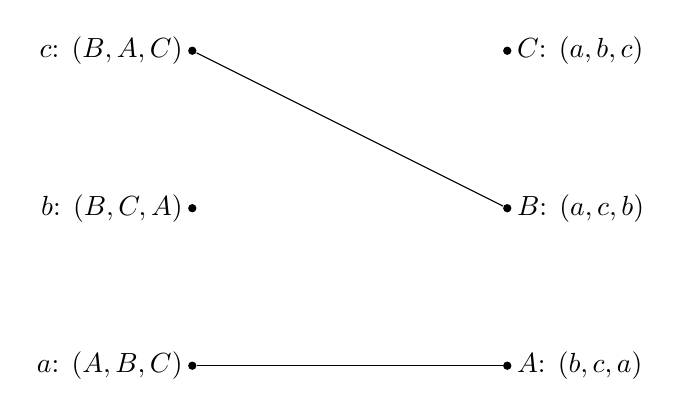
\begin{tikzpicture}[scale=2]
    \node (a) [end] at (0,0) {};
    \node (b) [end] at (0,1) {};
    \node (c) [end] at (0,2) {};
    \node (A) [end] at (2,0) {};
    \node (B) [end] at (2,1) {};
    \node (C) [end] at (2,2) {};
    \node [left] at (a) {$a$: $(A,B,C)$};
    \node [left] at (b) {$b$: $(B,C,A)$};
    \node [left] at (c) {$c$: $(B,A,C)$};
    \node [right] at (A) {$A$: $(b,c,a)$};
    \node [right] at (B) {$B$: $(a,c,b)$};
    \node [right] at (C) {$C$: $(a,b,c)$};
    \draw (a) -- (A);
    \draw (c) -- (B);
%    \draw (b) -- (C);
\end{tikzpicture}
    }

    \note{
        We pick \(b\) and as \(B\) is matched but prefers \(c\) to \(b\) we
        cross out \(B\) from \(b\)'s preferences:
    }

    \frame{
        \centering
        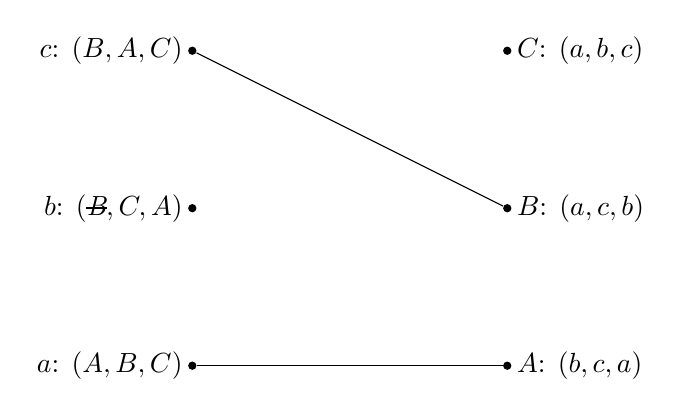
\begin{tikzpicture}[scale=2]
    \node (a) [end] at (0,0) {};
    \node (b) [end] at (0,1) {};
    \node (c) [end] at (0,2) {};
    \node (A) [end] at (2,0) {};
    \node (B) [end] at (2,1) {};
    \node (C) [end] at (2,2) {};
    \node [left] at (a) {$a$: $(A,B,C)$};
    \node [left] at (b) {$b$: $(\text{\textit{\sout{B}}},C,A)$};
    \node [left] at (c) {$c$: $(B,A,C)$};
    \node [right] at (A) {$A$: $(b,c,a)$};
    \node [right] at (B) {$B$: $(a,c,b)$};
    \node [right] at (C) {$C$: $(a,b,c)$};
    \draw (a) -- (A);
    \draw (c) -- (B);
%    \draw (b) -- (C);
\end{tikzpicture}
    }

    \note{
        We pick \(b\) again and set \(M(b)=C\).
    }

    \frame{
        \centering
        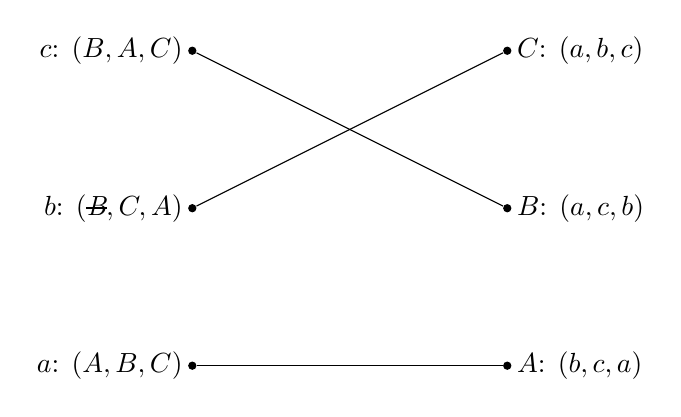
\begin{tikzpicture}[scale=2]
            \node (a) [end] at (0,0) {};
            \node (b) [end] at (0,1) {};
            \node (c) [end] at (0,2) {};
            \node (A) [end] at (2,0) {};
            \node (B) [end] at (2,1) {};
            \node (C) [end] at (2,2) {};
            \node [left] at (a) {$a$: $(A,B,C)$};
            \node [left] at (b) {$b$: $(\text{\textit{\sout{B}}},C,A)$};
            \node [left] at (c) {$c$: $(B,A,C)$};
            \node [right] at (A) {$A$: $(b,c,a)$};
            \node [right] at (B) {$B$: $(a,c,b)$};
            \node [right] at (C) {$C$: $(a,b,c)$};
            \draw (a) -- (A);
            \draw (c) -- (B);
            \draw (b) -- (C);
        \end{tikzpicture}
    }

        \note{And this final matching is in fact stable.}

\frame{
    \centering
    \includegraphics[height=.8\textheight]{./static/roth.jpg}

    \textbf{Alvin Roth}\footfullcite{roth1992} (1951 - )

    \tiny{By Bengt Nyman - Flickr: IMG\_4793, CC BY 2.0, https://commons.wikimedia.org/w/index.php?curid=23081905}
}

\note{
    Alvin Roth here actually shared the nobel Prize in economics with Shapley.

    He used matching games to design markets for organ exchange as well as
    school choice and medical internship.
}


\section{Routing Games}

\frame{
    \centering
\begin{tikzpicture}[scale=2, every node/.style={scale=2, draw,shape=circle, inner sep=.5pt, minimum size=.3cm}]
    \draw (0,0) node (s2) {\tiny{$s_2$}};
    \draw (0,1) node (s1) {\tiny{$s_1$}};
    \draw (2,.5) node (m1) {\tiny{$a$}};
    \draw (5,.5) node (t) {\tiny{$t$}};
    \draw [->] (s1) -- (m1);
    \draw [->] (s2) -- (m1);
    \draw [->] (m1) -- (t);
    \draw (s2) edge[out=-45,in=-135,->]  (t);
    \draw (s1) edge[out=45,in=135,->]  (t);
\end{tikzpicture}
}

\note{
    Here is another type of game. Imagine having an infinite amount of traffic
    that needs to get from the two sources here \(s_1, s_2\) to the sink \(t\).
    If of the roads (arcs on this network) have different amounts of congestion.
    Perhaps one of them is a road that can handle more traffic efficiently which
    makes it popular. Which in turn makes it slower.

    This is what is called a routing game.
}

\frame{
    \begin{definition}
        A \textbf{routing game} \((G,r,c)\) is defined on a graph \(G=(V,E)\) with a defined set of 
        sources \(s_i\) and sinks \(t_i\). 

        \begin{itemize}
            \item Each source-sink pair corresponds to a set of traffic 
        (also called a commodity) \(r_i\) that must travel along the edges of \(G\) from \(s_i\) to \(t_i\). 
            \item Every edge \(e\) of \(G\) has associated to it a nonnegative, continuous and nondecreasing 
        cost function (also called latency function) \(c_e\).
        \end{itemize}
    \end{definition}
}

\note{
    This is the formal definition of the routing game.
}

\frame{
    \begin{definition}
        For a routing game \((G,r,c)\) we define the optimal flow \(f^*\) as the
        solution to the following optimisation problem:

        \vspace{1cm}
        Minimise: \[\sum_{e\in E}c_e(f_e)f_e\]:

        Subject to:

        \[\begin{aligned}
            \sum_{P\in\mathcal{P}_i}f_P&=r_i&&\text{for all }i\\
            f_e&=\sum_{P\in\mathcal{P}\text{ if }e\in P}f_P&&\text{ for all }e\in E\\
            f_P&\geq 0
        \end{aligned}\]
    \end{definition}
}

\note{
    This is the formal definition of the optimal flow. Importantly, this is
    actually an easy problem mathematically (it's a convex optimisation
    problem).
}

\frame{
    For a routing game \((G,r,c)\) a flow \(\tilde f\) is called a 
    \textbf{Nash flow}
    if and only if for every commodity \(i\) and any two paths
    \(P_1,P_2\in\mathcal{P}_i\) such that \(f_{P_1}>0\) then:
    }

    \frame{
        \begin{definition}
            If \(c\) is a differentiable cost function then we define the
            \textbf{marginal cost} function \(c^*\) as:

            \[c^*=\frac{d}{dx}(xc(x))\]
        \end{definition}
    }

    \note{
        This however is the definition of a Nash flow.

        It is saying that if a particular path is used by traffic that that path
        must have minimal cost.

        This implies that the equilibrium is when all traffic is routed along
        minimal costing paths. In other words: no one has a reason to deviate.
    }

    \frame{
        \begin{theorem}{}
        For a routing game \((G,r,c)\) the Nash flow \(\tilde f\) is the
        solution to the following optimisation problem:

        \vspace{1cm}
        Minimise: \[\Phi(f)=\sum_{e\in E}\int_0^{f_e}c_e(x)dx\]:

        Subject to:

        \[\begin{aligned}
            \sum_{P\in\mathcal{P}_i}f_P&=r_i&&\text{for all }i\\
            f_e&=\sum_{P\in\mathcal{P}\text{ if }e\in P}f_P&&\text{ for all }e\in E\\
            f_P&\geq 0
        \end{aligned}\]
        \end{theorem}
    }

    \frame{
        \centering
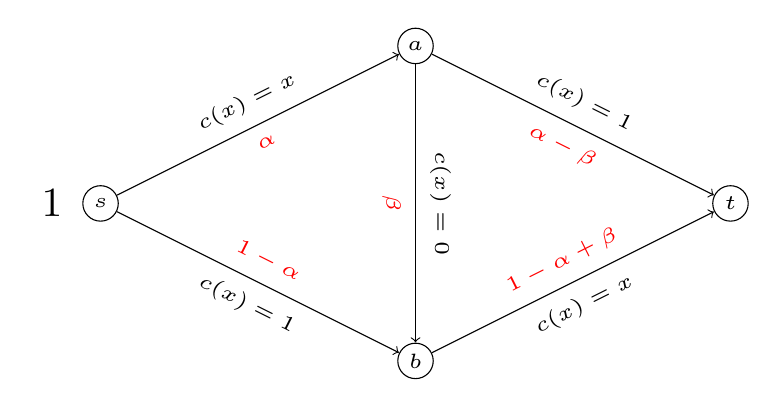
\begin{tikzpicture}[sloped, scale=2, every node/.style={scale=1.5}]
    \draw (-1,0) node[vertex] (s) {\tiny{$s$}};
    \draw (1,1) node[vertex] (a) {\tiny{$a$}};
    \draw (1,-1) node[vertex] (b) {\tiny{$b$}};
    \draw (3,0) node[vertex] (t) {\tiny{$t$}};
    \draw [->] (s) -- node [above] {\tiny{$c(x)=x$}} node [below,red] {\tiny{$\alpha$}} (a);
    \draw [->] (s) -- node [below] {\tiny{$c(x)=1$}} node [above,red] {\tiny{$1-\alpha$}} (b);
    \draw [->] (a) -- node [above] {\tiny{$c(x)=1$}} node [below,red] {\tiny{$\alpha-\beta$}} (t);
    \draw [->] (b) -- node [below] {\tiny{$c(x)=x$}} node [above,red] {\tiny{$1-\alpha+\beta$}} (t);
    \draw [->] (a) -- node [above]{\tiny{$c(x)=0$}} node [below,red] {\tiny{$\beta$}} (b);
    \node at (s) [left=.2cm] {$\tiny{1}$};
\end{tikzpicture}
    }

    \note{
        This is called Braess' Paradox.

        The optimal flow in this case is for half the flow to go along the top
        and half the flow to go along the bottom.

        The Paradox here is that by the addition of a resources (the super road)
        the congestion increases.

        There are real life examples of this: for example the Big Dig in Boston.
    }


\section{Cooperative Game Theory}

\frame{
    \centering
    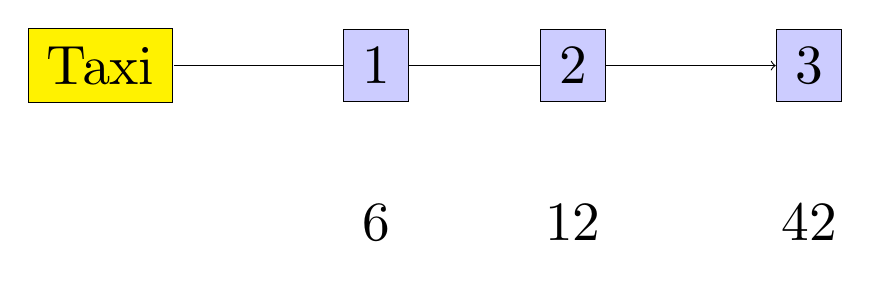
\begin{tikzpicture}[scale=2, every node/.style={scale=2}]
        \node (start) [draw,fill=yellow] {Taxi};
        \node (A) [draw,fill=blue!20!, right of=start, xshift=.75cm] {$1$};
        \node (B) [draw,fill=blue!20!, right of=start, xshift=2cm] {$2$};
        \node (C) [draw,fill=blue!20!, right of=start, xshift=3.5cm] {$3$};
        \node [below of=A] {6};
        \node [below of=B] {12};
        \node [below of=C] {42};
        \draw [->] (start) -- (A) -- (B) -- (C);
    \end{tikzpicture}
    }

    \note{
        Now for another type of game: how should these three people share a taxi
        fare?

        They have agreed to cooperate and now they want to know how to share
        their cost.
    }

\frame{
    \begin{definition}
        A \textbf{characteristic function game} \(G\) is given by a pair \((N,v)\) where
        \(N\) is the number of players and \(v:2^{[N]}\to\mathbb{R}\).     \end{definition}
    }

\note{
    Here is the characteristic function game for the taxi fare: how much would
    the fare be for each coalition of players:
    \[
        v(C)=\begin{cases}
            6,&\text{if }C=\{1\}\\
            12,&\text{if }C=\{2\}\\
            42,&\text{if }C=\{3\}\\
            12,&\text{if }C=\{1,2\}\\
            42,&\text{if }C=\{1,3\}\\
            42,&\text{if }C=\{2,3\}\\
            42,&\text{if }C=\{1,2,3\}\\
        \end{cases}
    \]
}

\frame{
    \Huge
    \begin{itemize}
        \item Efficiency;
        \item Null player;
        \item Symmetry;
        \item Additivity.
    \end{itemize}
    }

    \note{
        Is there a way to share out the fare in a way that matches these four
        axiomatic properties:

        \begin{itemize}
            \item The entire fare is paid.
            \item People who are not in the taxi do not pay.
            \item If people go the same distance they pay the same amount.
            \item It doesn't matter which taxi is taken.
        \end{itemize}
    }

\frame{
    \centering
    \includegraphics[height=.8\textheight]{./static/shapley.jpg}

    \textbf{Lloyd Shapley}\footfullcite{shapley1951} (1923 - 2016)


    \tiny{By Bengt Nyman - Flickr: IMG\_4826, CC BY 2.0, \url{https://commons.wikimedia.org/w/index.php?curid=23083494}}
}

\note{
    The answer is yes: Lloyd Shapley (him again) came up with an approach to do this.

    It is now referred to as the Shapley value.

}

\frame{
    Given \(G=(N,v)\) the \textbf{Shapley value} of player \(i\) is denoted by \(\phi_i(G)\) and given by:

\[\phi_i(G)=\frac{1}{N!}\sum_{\pi\in\Pi_n}\Delta_\pi^G(i)\]

where:


\[S_\pi(i)=\{j\in[N]\;|\;\pi(j)<\pi(i)\}\]

and 


\[\Delta_\pi^G(i)=v(S_{\pi}(i)\cup i)-v(S_{\pi}(i))\]
}

\frame{
    The Shapley value is the average vector that corresponds to the marginal
    contributions of each player in any given permutation of the players.

    Imagine letting people out of the taxi in random orders and they each pay
    what is owed at the time.
}

\frame{
    \centering
    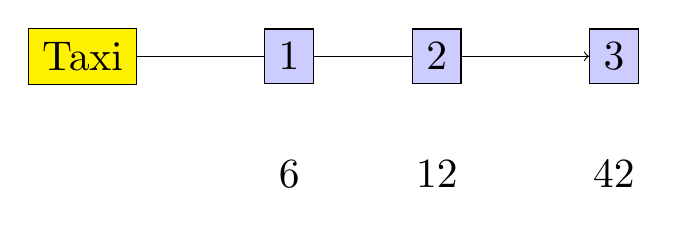
\begin{tikzpicture}[scale=1.5, every node/.style={scale=1.5}]
        \node (start) [draw,fill=yellow] {Taxi};
        \node (A) [draw,fill=blue!20!, right of=start, xshift=.75cm] {$1$};
        \node (B) [draw,fill=blue!20!, right of=start, xshift=2cm] {$2$};
        \node (C) [draw,fill=blue!20!, right of=start, xshift=3.5cm] {$3$};
        \node [below of=A] {6};
        \node [below of=B] {12};
        \node [below of=C] {42};
        \draw [->] (start) -- (A) -- (B) -- (C);
    \end{tikzpicture}

    \vspace{1cm}

\begin{tabular}{c|ccc}
    \toprule
    \(\pi\) & 1 & 2 & 3 \\
    \midrule
    \(1, 2, 3\) & 6 & 6 & 30\\
    \(1, 3, 2\) & 6 & 0 & 36\\
    \(2, 1, 3\) & 0 & 12 & 30\\
    \(2, 3, 1\) & 0 & 12 & 30\\
    \(3, 1, 2\) & 0 & 0 & 42\\
    \(3, 2, 1\) & 0 & 0 & 42\\
    \bottomrule
    Average     & 2 & 5 & 35\\
    \bottomrule
\end{tabular}
}

\note{
    Here is how that calculation looks here.

    We consider each permutation of the players and work out what they pay in
    that order.
}

\frame{

    \frametitle{Explainable AI\footfullcite{lundberg2017}}


    \centering
\begin{tabular}{c|c}
    Model      &                        \(R^2\)\\
    \midrule
    \(y=c_1x_1\)                   &0.075\\
    \(y=         c_2x_2\)          &0.086\\
    \(y=                  c_3x_3\) &0.629\\
    \(y=c_1x_1 + c_2x_2\)          &0.163\\
    \(y=c_1x_1          + c_3x_3\) &0.63\\
    \(y=         c_2x_2 + c_3x_3\) &0.906\\
    \(y=c_1x_1 + c_2x_2 + c_3x_3\) &0.907\\
\end{tabular}

\vspace{1cm}

\[\phi(G)=(0.0383, 0.1818, 0.6868)\]
}

\note{
    Here is another example application.

    In this simple version of `AI' (it's just fitting a linear function to some
    data) we can try to see the effect each variable makes. What explains the
    contribution more?

    \(R^2\) is a measure of explained variability in a given model.

    The Shapley value can be used here to see how best to attribute the total
    \(R^2\).
}

\frame{
    \begin{center}
        \Large
        \url{daffidwilde.github.io/matching/}

        \url{coopgt.readthedocs.io}

        \url{knightva@cardiff.ac.uk}
    \end{center}
}

\note{Here are some examples of good pieces of software with good documentation
for all of the above (except for the routing games.)}

\end{document}
